\documentclass[12pt, a4paper]{scrreprt}
\usepackage[margin=2.5cm]{geometry}
\usepackage[hidelinks]{hyperref}
\usepackage{graphicx,xcolor,listings,tikz,enumitem}
\usetikzlibrary{positioning, arrows.meta, shapes, fit}

\definecolor{codegreen}{rgb}{0,0.6,0}
\definecolor{codegray}{rgb}{0.5,0.5,0.5}
\definecolor{codepurple}{rgb}{0.58,0,0.82}
\definecolor{backcolour}{rgb}{0.95,0.95,0.92}

\lstdefinestyle{mystyle}{
  backgroundcolor=\color{backcolour},
  commentstyle=\color{codegreen},
  keywordstyle=\color{blue},
  stringstyle=\color{codepurple},
  basicstyle=\ttfamily\footnotesize,
  numbers=left,
  numbersep=5pt,
  breaklines=true,
  tabsize=2
}
\lstset{style=mystyle}

\newcommand{\faculty}{Faculty Applied Information Technology}
\newcommand{\studies}{Bachelor of Cyber-Security}
\newcommand{\thesistitleDE}{Projekt "WeedDetector" \\ Projektübergabe}
\newcommand{\submissiondate}{05.\ Juli 2025}
\newcommand{\supervisor}{Prof.\ Dr.\ Holger Jehle}

\begin{document}

\begin{titlepage}
  \centering
  {\LARGE Technische Hochschule Deggendorf \\ \faculty \par}
  \vspace{0.3cm}
  {\Large Studiengang \studies \\[1.5cm]}
  {\Huge\bfseries \thesistitleDE\par}
  \vfill
  \begin{minipage}[t]{0.45\textwidth}
    \textbf{Vorgelegt von:}\\
    \\
    Christof Renner (22301943)\\
    Manuel Friedl (1236626)\\
    \\
    \\
    \\
    \\
    Datum: \submissiondate
  \end{minipage}\hfill
  \begin{minipage}[t]{0.45\textwidth}
    \textbf{Prüfungsleitung:}\\
    \\
    \supervisor
  \end{minipage}
\end{titlepage}

\tableofcontents
\newpage

\chapter{Einführung und Projektübersicht}

\section{Motivation und Zielsetzung}
Der \textbf{WeedDetector} ist ein innovatives Softwaresystem, das entwickelt wurde, um in landwirtschaftlichen Umgebungen automatisiert Unkräuter zu erkennen und zu klassifizieren. Die Hauptmotivation hinter diesem Projekt liegt in der zunehmenden Notwendigkeit nachhaltiger landwirtschaftlicher Praktiken und der Reduzierung des Einsatzes von Herbiziden.

Dieses Projekt entstand aus folgenden konkreten Anforderungen:
\begin{itemize}
    \item \textbf{Präzisionslandwirtschaft:} Durch die genaue Identifikation von Unkraut können Landwirte gezielt eingreifen, anstatt flächendeckend Herbizide einzusetzen.
    \item \textbf{Umweltschutz:} Reduzierung des Chemikalieneinsatzes durch punktgenaue Behandlung von Unkrautflächen.
    \item \textbf{Automatisierung:} Integration mit Robotersystemen zur vollautomatischen Unkrautbekämpfung.
    \item \textbf{Kosteneinsparung:} Verringerung des Ressourcenverbrauchs und effizientere Arbeitsabläufe.
\end{itemize}

\section{Systemarchitektur}
Der WeedDetector folgt dem Model-View-Controller (MVC) Architekturmuster, um eine saubere Trennung der Verantwortlichkeiten zu gewährleisten und die Wartbarkeit zu verbessern.

\begin{figure}[h!]
    \centering
    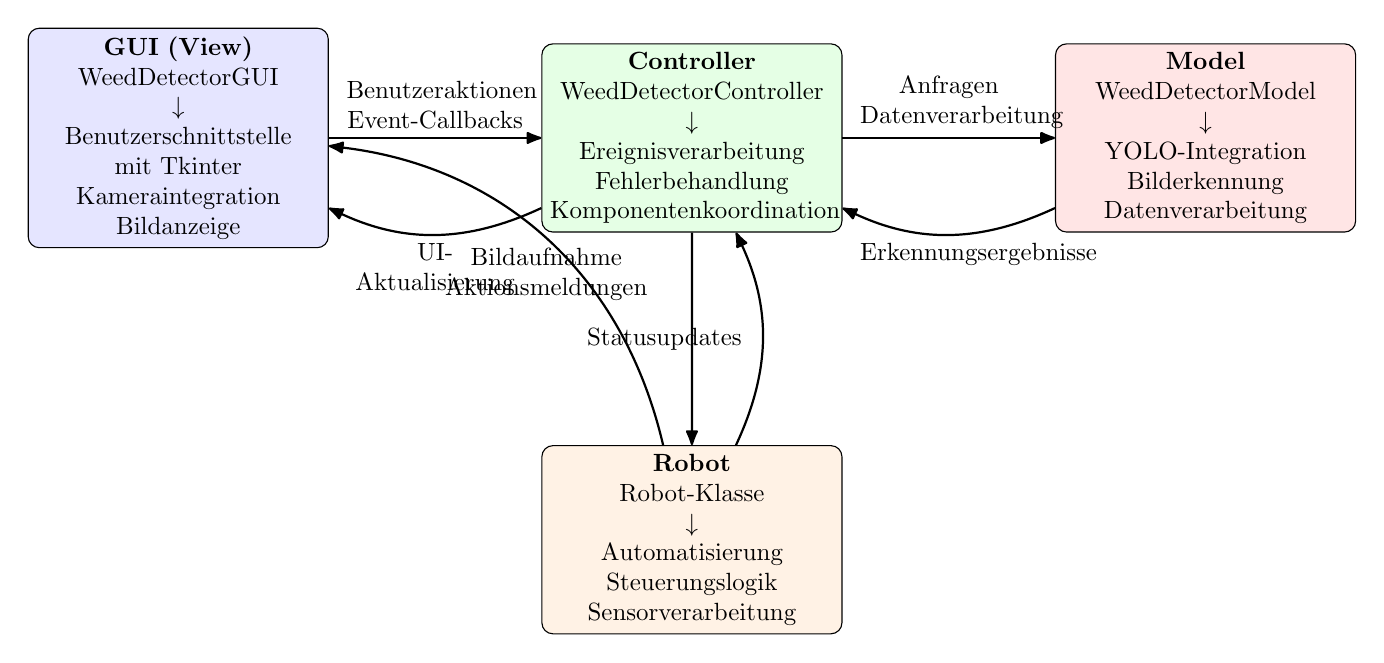
\begin{tikzpicture}[
        scale= 0.9,
        transform shape,
        node distance=3 cm and 3cm,
        box/.style={draw, text width=4cm, align=center, rounded corners, minimum height=2cm},
        arrow/.style={draw, thick, -{Latex[round]}}
    ]

    % Hauptkomponenten
    \node (gui) [box, fill=blue!10] {\textbf{GUI (View)}\\WeedDetectorGUI\\$\downarrow$\\Benutzerschnittstelle mit Tkinter\\Kameraintegration\\Bildanzeige};
    
    \node (controller) [box, right=of gui, fill=green!10] {\textbf{Controller}\\WeedDetectorController\\$\downarrow$\\Ereignisverarbeitung\\Fehlerbehandlung\\Komponentenkoordination};
    
    \node (model) [box, right=of controller, fill=red!10] {\textbf{Model}\\WeedDetectorModel\\$\downarrow$\\YOLO-Integration\\Bilderkennung\\Datenverarbeitung};
    
    \node (robot) [box, below=of controller, fill=orange!10] {\textbf{Robot}\\Robot-Klasse\\$\downarrow$\\Automatisierung\\Steuerungslogik\\Sensorverarbeitung};

    % Verbindungen
    \draw[arrow] (gui) -- node[above, text width=2.5cm, align=center] {Benutzeraktionen\\Event-Callbacks} (controller);
    \draw[arrow] (controller) -- node[above, text width=2.5cm, align=center] {Anfragen\\Datenverarbeitung} (model);
    \draw[arrow] (model) to[bend left=25] node[below, text width=2.5cm, align=center] {Erkennungsergebnisse} (controller);
    \draw[arrow] (controller) to[bend left=25] node[below, text width=2.5cm, align=center] {UI-Aktualisierung} (gui);
    \draw[arrow] (controller) -- node[right, text width=2.5cm, align=center] {} (robot);
    \draw[arrow] (robot) to[bend right=25] node[left, text width=2.5cm, align=center] {Statusupdates} (controller);
    \draw[arrow] (robot) to[bend right=35] node[below, text width=3.5cm, align=center] {Bildaufnahme\\Aktionsmeldungen} (gui);

    \end{tikzpicture}
    \caption{Detaillierte Architektur des WeedDetector-Systems}
    \label{fig:systemarchitektur}
\end{figure}

\section{Technologiestack}
Der WeedDetector nutzt einen modernen Technologiestack, der für Bildverarbeitung und maschinelles Lernen optimiert ist:

\begin{itemize}
    \item \textbf{Programmiersprache:} Python 3.13 als Hauptsprache für die gesamte Anwendung
    \item \textbf{Computer Vision:}
    \begin{itemize}
        \item OpenCV 4.11.0.86 für Bildverarbeitung und Kameraintegration
        \item Ultralytics YOLOv8 8.3.155 für Objekterkennung und -klassifikation
    \end{itemize}
    \item \textbf{Benutzeroberfläche:}
    \begin{itemize}
        \item Tkinter für die grafische Benutzeroberfläche
        \item Pillow 11.2.1 für erweiterte Bildverarbeitung in der GUI
    \end{itemize}
    \item \textbf{Containerisierung:} Docker für einheitliche Entwicklungs- und Produktionsumgebungen
    \item \textbf{Kontinuierliche Integration:} GitHub Actions für automatisierte Tests und Builds
\end{itemize}

\chapter{Installation und Konfiguration}

\section{Systemvoraussetzungen}
Für den erfolgreichen Betrieb des WeedDetector-Systems werden folgende Mindestsystemvoraussetzungen empfohlen:

\begin{itemize}
    \item \textbf{Hardware:}
    \begin{itemize}
        \item CPU: Quad-Core Prozessor, 2.5 GHz oder höher
        \item RAM: Mindestens 8 GB (16 GB empfohlen)
        \item Grafikkarte: GPU mit mindestens 4 GB VRAM für optimale Leistung
        \item Festplattenspeicher: Mindestens 10 GB freier Speicherplatz
        \item Kamera: USB-Webcam oder integrierte Kamera für Live-Erkennung
    \end{itemize}
    \item \textbf{Software:}
    \begin{itemize}
        \item Betriebssystem: Linux (Ubuntu 22.04 LTS empfohlen), Windows 10/11 oder macOS
        \item Docker: Version 24.0 oder höher
    \end{itemize}
\end{itemize}

\section{Installationsanleitung}
Die Installation des WeedDetector-Systems erfolgt primär über Docker, um eine konsistente Umgebung zu gewährleisten und Abhängigkeitsprobleme zu vermeiden.

\subsection{Installation mittels Docker}
\begin{enumerate}
    \item \textbf{Docker installieren:} Falls noch nicht geschehen, installieren Sie Docker gemäß der offiziellen Anleitung für Ihr Betriebssystem (\url{https://docs.docker.com/get-docker/}).
    
    \item \textbf{Repository klonen:}
    \begin{lstlisting}[language=bash]
    git clone https://github.com/SS25-SoftwareEngineering-WeedDetector.git
    cd SS25-SoftwareEngineering-WeedDetector
    \end{lstlisting}
    
    \item \textbf{Docker-Image erstellen:}
    \begin{lstlisting}[language=bash]
    docker build -t weed-detector .
    \end{lstlisting}
    
    \item \textbf{Anwendung starten:}
    \begin{lstlisting}[language=bash]
    docker run --device /dev/video0:/dev/video0 --net=host -e DISPLAY=$DISPLAY -v /tmp/.X11-unix:/tmp/.X11-unix weed-detector
    \end{lstlisting}
\end{enumerate}

\subsection{Manuelle Installation für Windows (ohne Docker)}
Für Entwicklungs- oder Testzwecke unter Windows muss das System über Python direkt:

\begin{enumerate}
    \item \textbf{Python-Umgebung einrichten:}
    \begin{lstlisting}[language=bash]
    python -m venv venv
    source venv/bin/activate  # Unter Windows: venv\Scripts\activate
    \end{lstlisting}
    
    \item \textbf{Abhängigkeiten installieren:}
    \begin{lstlisting}[language=bash]
    pip install -r requirements.txt
    \end{lstlisting}
    
    \item \textbf{Anwendung starten:}
    \begin{lstlisting}[language=bash]
    python app/main.py
    \end{lstlisting}
\end{enumerate}

\section{Konfiguration und Anpassung}
Der WeedDetector bietet verschiedene Konfigurationsmöglichkeiten, um das System an spezifische Anforderungen anzupassen:

\subsection{Modellkonfiguration}
Die Standardkonfiguration verwendet ein vortrainiertes YOLO-Modell. Das System sucht automatisch nach trainierten Modellen in folgenden Pfaden:
\begin{itemize}
    \item \texttt{runs/detect\_train/weights/best.pt}
    \item \texttt{data/weights/best.pt}
    \item \texttt{data/models/best.pt}
    \item \texttt{models/best.pt}
\end{itemize}

Wenn kein benutzerdefiniertes Modell gefunden wird, wird auf das Standard-YOLO-Modell zurückgegriffen.

\subsection{Umgebungsvariablen}
Folgende Umgebungsvariablen können beim Start des Docker-Containers konfiguriert werden:
\begin{itemize}
    \item \texttt{QT\_X11\_NO\_MITSHM=1}: Verhindert Probleme mit X11-Shared-Memory
    \item \texttt{QT\_DEBUG\_PLUGINS=1}: Aktiviert Debug-Ausgaben für Qt-Plugins
    \item \texttt{OPENCV\_VIDEOIO\_PRIORITY\_V4L2=0}: Priorität für Video4Linux2-Backend
    \item \texttt{OPENCV\_VIDEOIO\_DEBUG=1}: Aktiviert Debug-Informationen für OpenCV Video-I/O
\end{itemize}

\chapter{Milestones \& User Stories}
In diesem Abschnitt werden die wichtigsten \textbf{Meilensteine} und \textbf{User Stories} des Projekts Weed Detector dokumentiert. Sie dienen dazu, den Projektfortschritt nachvollziehbar zu machen und zeigen auf, wie die Anforderungen schrittweise umgesetzt wurden.\\
\\
Die User Stories orientieren sich an den Bedürfnissen der Nutzer und definieren die Funktionen aus Anwendersicht, während die Milestones die wesentlichen Etappen im Entwicklungsprozess markieren, um die Struktur und Planung des Projekts übersichtlich darzustellen.

\section{Milestones}
Folgende Meilensteine wurden am Anfang des Projektes festgelegt:
\begin{enumerate}
    \item \textbf{Anforderungsanalyse \& Architektur (05.05. - 12.05.25):} Festlegen des technischen Konzepts und der Architektur
    \item \textbf{Prototyp Klassifikation \& Koordinatenbestimmung (12.05. - 25.05.25):} Passenden Datensatz (Bilder, WeedAI) suchen oder erstellen, Bilder in ein einheitliches Format bringen, labeln und optional durch Data Augmentation erweitern.
    \item \textbf{Prototyp Navigation \& Integration (25.05. - 08.06.25):} Implementierung der Bildvorverarbeitung, Klassifikation und Koordinatenbestimmung sowie erste Integration in ROS.
    \item \textbf{Test, Validierung \& Performance-Optimierung (08.06. - 22.06.25):} Erstellung und Durchführung von Unit-, Integrations- und Performance-Tests
    \item \textbf{Dokumentation \& Präsentation (22.06. - 07.07-25):} Dokumentation (Ziele, Methodik, Ergebnisse) erstellen, Code kommentieren, Screenshots einfügen, Präsentation vorbereiten und am 07.07.25 präsentieren.
\end{enumerate}

\section{User Stories}
Nachfolgend werden die User Stories aufgeführt, die zu den jeweiligen Milestones definiert wurden, um die Anforderungen aus Nutzersicht klar darzustellen und den Bezug zum Entwicklungsfortschritt sichtbar zu machen.\\
\begin{itemize}
    \item \textbf{M1:}
    \begin{itemize}
        \item Als \emph{Entwickler} möchte ich Anforderungen und Ziele definieren, um eine klare Projektvision zu haben.
        \item Als \emph{Entwickler} möchte ich die passenden Tools und Bibliotheken auswählen, um den Entwicklungsprozess effizient zu gestalten.
    \end{itemize}
    \item \textbf{M2:}
    \begin{itemize}
        \item Als \emph{Landwirt/Gärtner} möchte ich, dass der Weeds Detector typische Unkräuter erkennt, um mein Feld effizient zu analysieren.
        \item Als \emph{Entwickler} möchte ich ein ML-Modell trainieren, das Unkraut in Bildern erkennt, um den Erkennungsprozess zu automatisieren.
        \item Als \emph{Entwickler} möchte ich die Koordinaten der Unkrautpositionen berechnen, um die Lokalisierung zu ermöglichen.
        \item ALs \emph{User} möchte ich, dass das System visuell anzeigt, wo Unkraut erkannt wurde, damit ich gezielt eingreifen kann.
    \end{itemize}
    \item \textbf{M3:}
    \begin{itemize}
        \item Als \emph{Landwirt/Gärtner} möchte ich, dass der Roboter zielgerichtet zum Unkraut fährt, um manuelles Eingreifen zu reduzieren.
        \item Als \emph{Entwickler} möchte ich erkannte Koordinaten an das Navigationssystem übergeben, damit gezielt darauf reagiert werden kann.
        \item Als \emph{Entwickler} möchte ich Navigation und Klassifikation integrieren, um ein durchgängiges System zu schaffen.
    \end{itemize}
    \item \textbf{M4:}
    \begin{itemize}
        \item Als \emph{Nutzer} möchte ich wissen, wie zuverlässig die Vorhersagen sind, um Vertrauen ins System zu haben.
        \item Als \emph{Nutzer} möchte ich die Anwendung einfach und selbsterklärend bedienen können.
        \item Als \emph{Entwickler} möchte ich das Modell mit neuen Bildern testen, um die Genauigkeit zu validieren.
    \end{itemize}
    \item \textbf{M5:}
    \begin{itemize}
        \item Als \emph{Stakeholder} möchte ich verstehen, wie das System funktioniert, um seine Relevanz zu beurteilen.
        \item Als \emph{Entwickler} möchte ich meinen Code und Ergebnisse dokumentieren, um das Projekt verständlich und nachvollziehbar zu machen.
        \item Als \emph{Entwickler} möchte ich eine Präsentation vorbereiten, um mein Projekt überzeugend vorstellen zu können
    \end{itemize}
\end{itemize}

\chapter{Scope Changes \& Blocking Issues}

\section{Scope Changes}
In diesem Abschnitt werden die \textbf{Änderungen am ursprünglichen Projektumfang (Scope Changes)} dokumentiert, die im Verlauf der Entwicklung notwendig wurden. Diese Anpassungen entstanden durch neue Anforderungen, technische Herausforderungen oder Optimierungsmöglichkeiten und zeigen, wie das Projekt flexibel an veränderte Bedingungen angepasst wurde.
\begin{itemize}
    \item \textbf{Meilenstein 2:} Festlegung, dass der Docker-Container nur unter Linux läuft, um Kompatibilitätsprobleme mit der Tkinter-Library unter Windows zu vermeiden.
    \item \textbf{Meilenstein 3:} Ergänzung eines UI end-to-end Redesign \& Refactors, um eine seamless UI/UX und zeitgemäße Ästhetik gemäß Best Practices sicherzustellen.
\end{itemize}

\section{Blocking Issues}
Im Verlauf des Projekts traten keine direkten \textbf{Blocking Issues} auf, die den Fortschritt maßgeblich verzögert oder die Entwicklung gestoppt hätten. Alle auftretenden technischen oder organisatorischen Herausforderungen konnten zeitnah identifiziert und gelöst werden, wodurch ein kontinuierlicher Arbeitsfluss im Projekt gewährleistet war.

\chapter{Modelltraining und -anpassung}

\section{Vorbereitung des Trainingsdatensatzes}
Die Qualität des Erkennungsmodells hängt maßgeblich von der Qualität und Vielfalt des Trainingsdatensatzes ab.

\subsection{Datenannotation}
Die Annotation der Trainingsdaten kann mit folgenden Tools durchgeführt werden:
\begin{itemize}
    \item \textbf{Roboflow:} Online-Plattform mit intuitiver Benutzeroberfläche
    \item \textbf{LabelImg:} Lokales Open-Source-Tool für YOLO-Annotationen
    \item \textbf{CVAT:} Leistungsstarkes webbasiertes Annotationstool
\end{itemize}

\subsection{Datenaugmentierung}
Zur Verbesserung der Modellrobustheit werden folgende Augmentierungstechniken empfohlen:
\begin{itemize}
    \item Horizontale und vertikale Spiegelung
    \item Rotation (±15° bis ±90°)
    \item Zufällige Zuschnitte (0-20\%)
    \item Helligkeits- und Kontrastvariationen (±10-20\%)
    \item Sättigungsanpassungen (±20\%)
\end{itemize}

\section{Durchführung des Trainings}
Der Trainingsprozess kann sowohl lokal als auch in der Cloud durchgeführt werden.

\subsection{Training starten}
Starten Sie das Training mit dem folgenden Befehl:
\begin{lstlisting}[language=bash]
python train.py --data data/data.yaml --epochs 50 --img 640 --batch 16
\end{lstlisting}

Trainingsparameter können je nach verfügbarer Hardware angepasst werden:
\begin{itemize}
    \item \texttt{--epochs}: Anzahl der Trainingsdurchläufe (empfohlen: 50-300)
    \item \texttt{--img}: Bildgröße für das Training (empfohlen: 640)
    \item \texttt{--batch}: Batch-Größe (an verfügbaren GPU-Speicher anpassen)
\end{itemize}

\section{Modellbewertung und -optimierung}
Nach Abschluss des Trainings sollte das Modell bewertet und optimiert werden.

\subsection{Bewertungsmetriken}
Die wichtigsten Metriken zur Bewertung des Modells sind:
\begin{itemize}
    \item \textbf{mAP (mean Average Precision):} Gesamtgenauigkeit über alle Klassen
    \item \textbf{Precision:} Verhältnis korrekter Erkennungen zu allen Erkennungen
    \item \textbf{Recall:} Verhältnis korrekter Erkennungen zu allen tatsächlichen Objekten
    \item \textbf{F1-Score:} Harmonisches Mittel aus Precision und Recall
\end{itemize}

\subsection{Feinabstimmung des Modells}
Bei unzureichender Leistung können folgende Optimierungsschritte durchgeführt werden:
\begin{enumerate}
    \item \textbf{Daten verbessern:} Mehr Trainingsbilder, bessere Annotation, zusätzliche Augmentierung
    \item \textbf{Hyperparameter anpassen:} Lernrate, Epochenzahl, Batch-Größe
    \item \textbf{Modellarchitektur ändern:} Größeres/kleineres Basismodell (YOLOv8n, YOLOv8s, YOLOv8m, YOLOv8l, YOLOv8x)
    \item \textbf{Transfer Learning:} Training auf vortrainiertem Modell für verwandte Domänen
\end{enumerate}

\section{Fehlerbehandlung und Logging}
Das System implementiert eine umfassende Fehlerbehandlung, um Robustheit zu gewährleisten:

\begin{itemize}
    \item \textbf{Exception Handling:} Alle kritischen Operationen sind mit spezifischen Exception-Handlern umgeben.
    \item \textbf{Fehlerprotokolle:} Fehler werden sowohl in der Konsole als auch in der GUI angezeigt.
    \item \textbf{Fallback-Mechanismen:} Bei Problemen mit benutzerdefinierten Modellen erfolgt ein Fallback auf das Standardmodell.
    \item \textbf{Robuste Kameraintegration:} Sichere Behandlung von Kamerazugriffsfehlern und Bildverarbeitungsproblemen.
\end{itemize}

\chapter{Test, Validierung \& Perfromance-Optimierung}

\section{Unit-, Integration- und Systemtests}
\subsection{Unit-Tests}
Für die Weed Detector Anwendung wurden umfangreiche Unittests entwickelt, um die Funktionalität und Stabilität der wichtigsten Komponenten sicherzustellen. Die Tests decken insbesondere die grafische Benutzeroberfläche (GUI), das Modell zur Unkrauterkennung sowie die Controller-Logik ab. Dabei werden sowohl typische Anwendungsfälle als auch Fehler- und Randfälle überprüft. Die GUI-Tests simulieren Benutzerinteraktionen wie das Auswählen und Anzeigen von Bildern, das Starten und Stoppen der Kamera sowie das Anzeigen von Fehlermeldungen. Für das Modell werden unter anderem das Laden und Verarbeiten von Bildern, die Fehlerbehandlung bei ungültigen Dateien und die Formatierung der Erkennungsergebnisse getestet. Die Controller-Tests prüfen das Zusammenspiel zwischen GUI und Modell, einschließlich der Fehlerbehandlung und der Steuerung des Roboters. Durch den Einsatz von Mocking werden externe Abhängigkeiten isoliert, sodass die Tests reproduzierbar und unabhängig von der Hardware ausgeführt werden können. Die Unittests tragen maßgeblich zur Qualitätssicherung und Wartbarkeit des Projekts bei.\\

\begin{lstlisting}[language=Python, caption=Beispiel Unit-Test]
    @patch('tkinter.messagebox.showerror')
    def test_show_error_box(self, mock_showerror):
        """Test if error box is shown correctly."""
        self.gui.show_error_box("Fehlertext")
        mock_showerror.assert_called_with("Error", "Fehlertext")
        content = self.gui.results_text.get("1.0", tk.END)
        self.assertIn("Error: Fehlertext", content)
    \end{lstlisting}

\subsection{Integrations-Tests}
Zur Sicherstellung des fehlerfreien Zusammenspiels aller Hauptkomponenten wurden für die Weed Detector Anwendung umfassende Integrationstests implementiert. Diese Tests überprüfen insbesondere die Interaktion zwischen GUI, Modell und Controller im Gesamtsystem. Es werden typische Abläufe wie das Laden und Verarbeiten von Bildern, die Anzeige von Ergebnissen, das Starten und Stoppen des Roboters sowie die Fehlerbehandlung bei fehlerhaften Eingaben getestet. Dabei wird sowohl das Verhalten bei korrekten als auch bei fehlerhaften Abläufen geprüft, um die Robustheit der Anwendung zu gewährleisten. Durch den Einsatz von Mocks für GUI-Elemente und Modellfunktionen können die Integrationstests unabhängig von externer Hardware und realen Bilddaten ausgeführt werden. Die Integrationstests tragen somit entscheidend dazu bei, die Zuverlässigkeit und Stabilität der gesamten Anwendung sicherzustellen.\\

\begin{lstlisting}[language=Python, caption= Beispiel Integrations-Test]
    def test_model_detect_weeds_with_real_image(self):
        """Test: mnodel detects weeds and returns results."""
        image_path = os.path.join(os.path.dirname(__file__), "..", "unkraut1.jpg")
        image_path = os.path.abspath(image_path)
        if not os.path.exists(image_path):
            self.skipTest("unkraut1.jpg not found")
        image = cv2.imread(image_path)
        processed, result = self.model.detect_weeds(image)
        self.assertIsNotNone(processed)
        self.assertIsInstance(result, str)
    \end{lstlisting}

\subsection{Systemtest}
Für die Weed Detector Anwendung wurde ein Systemtest implementiert, der den vollständigen Ablauf der Unkrauterkennung unter realistischen Bedingungen simuliert. Dabei werden alle Hauptkomponenten – Modell, GUI und Controller – gemeinsam in einer Testumgebung ausgeführt. Der Test bildet einen typischen Nutzer-Workflow ab: Ein reales Bild wird geladen, durch das Modell verarbeitet und das Ergebnis anschließend in der grafischen Oberfläche angezeigt. Abschließend wird überprüft, ob die Erkennungsergebnisse korrekt im GUI dargestellt werden. Dieser End-to-End-Test stellt sicher, dass die Integration aller Komponenten im Gesamtsystem funktioniert und die Anwendung aus Sicht eines Anwenders zuverlässig arbeitet. Der Systemtest trägt somit wesentlich zur Qualitätssicherung und zur Validierung der zentralen Funktionalität der Anwendung bei.\\

\begin{lstlisting}[language=Python, caption=Code-Snippet Systemtest]
    ...
    def test_full_detection_flow(self):
        """Simulate user uploading an image and verify detection and GUI update."""
        # Simulate user selects image
        image = self.model.load_image(self.image_path)
        processed, result = self.model.detect_weeds(image)
        # Display in GUI
        self.gui.display_image(processed)
        self.gui.update_results(result)
        # Check that results are shown in the GUI
        gui_content = self.gui.results_text.get("1.0", "end")
        self.assertIn("weed", gui_content.lower())
        self.assertGreater(len(gui_content.strip()), 0)
    ...
    \end{lstlisting}

\newpage


\section{Line Coverage}
Zur Sicherstellung der Codequalität wurde die Line-Coverage des Projekts gemessen, um die Abdeckung der implementierten Unit- und Integrationstests zu überprüfen. Der Weed Detector erreichte dabei eine \textbf{Total Coverage Score von 85\%}, was eine hohe Testabdeckung widerspiegelt und zeigt, dass der Großteil des Codes durch Tests abgesichert ist.\\

\begin{lstlisting}[language=Bash, caption=Line Coverage]
PS C:\Repos\SS25-SoftwareEngineering-WeedDetector> python -m coverage report
    Name                Stmts   Miss  Cover
    ---------------------------------------
    app\controller.py      55      6    89%
    app\gui.py            231     32    86%
    app\main.py            10      1    90%
    app\model.py          112     19    83%
    app\robot.py           45      9    80%
    ---------------------------------------
    TOTAL                 453     67    85%
\end{lstlisting}

\section{Linting}
Zur Sicherstellung einer sauberen und einheitlichen Codebasis wurde im Projekt Pylint für Linting eingesetzt. Der gesamte Code des Weed Detectors wurde damit auf Syntaxfehler, Stilkonformität nach PEP8 und potenzielle Probleme geprüft.\\
\\
Durch regelmäßiges Linting konnte die Codequalität verbessert, die Lesbarkeit erhöht und die Wartbarkeit des Projekts sichergestellt werden.\\

\begin{lstlisting}[language=Bash, caption=Pylint Score]
    -----------------------------------
    Your code has been rated at 8.97/10
\end{lstlisting} 


\chapter{Wartung und Weiterentwicklung}

\section{Bekannte Einschränkungen}
Das aktuelle System hat folgende bekannte Einschränkungen:

\begin{itemize}
    \item \textbf{Rechenleistung:} Die Echtzeiterkennung benötigt ausreichende CPU/GPU-Ressourcen.
    \item \textbf{Lichtempfindlichkeit:} Die Erkennungsgenauigkeit variiert je nach Lichtverhältnissen.
    \item \textbf{Modellspezifität:} Das Modell funktioniert am besten für die Unkrautarten, auf die es trainiert wurde.
    \item \textbf{GUI-Beschränkungen:} Die Tkinter-Oberfläche hat eingeschränkte Anpassungsmöglichkeiten.
\end{itemize}

\section{Erweiterungsmöglichkeiten}
Folgende Erweiterungen sind für zukünftige Versionen geplant:

\begin{enumerate}
    \item \textbf{Erweiterte Roboterintegration:} Unterstützung für komplexere Roboterhardware und -steuerung.
    \item \textbf{Cloud-Integration:} Anbindung an Cloud-Dienste für Modelltraining und Datenspeicherung.
    \item \textbf{Mehrsprachige Unterstützung:} Internationalisierung der Benutzeroberfläche.
    \item \textbf{Mobile App:} Entwicklung einer begleitenden mobilen Anwendung für Felddiagnosen.
    \item \textbf{Kartenintegration:} Geo-Tagging und Kartierung erkannter Unkrautbereiche.
    \item \textbf{Verbesserte Bildvorverarbeitung:} Automatische Bildkorrektur für verschiedene Lichtverhältnisse.
\end{enumerate}

\section{Wartungsrichtlinien}
Zur langfristigen Wartung der Anwendung sollten folgende Richtlinien beachtet werden:

\begin{itemize}
    \item \textbf{Regelmäßige Updates:} Aktualisierung der Abhängigkeiten, insbesondere von OpenCV und YOLOv8.
    \item \textbf{Modellneuevaluierung:} Periodische Neubewertung und ggf. Neutraining des Erkennungsmodells.
    \item \textbf{Codeüberprüfung:} Regelmäßige statische Codeanalyse mit Bandit, Snyk und Pylint.
    \item \textbf{Dokumentationsaktualisierung:} Aktualisierung der Dokumentation bei Änderungen am Code oder an Funktionen.
    \item \textbf{Testabdeckung:} Aufrechterhaltung und Erweiterung der automatisierten Testabdeckung.
\end{itemize}

\chapter{Fazit und Ausblick}

\section{Projektergebnisse}
Der WeedDetector repräsentiert eine erfolgreiche Integration moderner Computer-Vision-Technologien in landwirtschaftliche Anwendungen. Das System bietet:

\begin{itemize}
    \item Eine benutzerfreundliche Oberfläche für die Unkrauterkennung
    \item Ein anpassbares und erweiterbares YOLO-basiertes Erkennungsmodell
    \item Eine modulare, wartbare Architektur nach dem MVC-Muster
    \item Eine vollständige Containerisierung für einfache Bereitstellung
\end{itemize}

\section{Zukünftige Forschungsrichtungen}
Basierend auf den Erfahrungen aus diesem Projekt ergeben sich folgende zukünftige Forschungs- und Entwicklungsrichtungen:

\begin{enumerate}
    \item \textbf{Multi-Spektralanalyse:} Integration von Infrarot- und Multispektraldaten für verbesserte Erkennung.
    \item \textbf{Drohnenintegration:} Anpassung des Systems für den Einsatz auf landwirtschaftlichen Drohnen.
    \item \textbf{Federated Learning:} Verteiltes Modelltraining zwischen verschiedenen landwirtschaftlichen Betrieben.
    \item \textbf{Präzisionssprühmechanismen:} Entwicklung präziser Mechanismen zur gezielten Behandlung einzelner Unkrautpflanzen.
    \item \textbf{Langzeitüberwachung:} Systeme zur kontinuierlichen Überwachung und Analyse der Unkrautentwicklung über Wachstumsperioden hinweg.
\end{enumerate}

\section{Abschließende Bewertung}
Der WeedDetector stellt einen bedeutenden Schritt in Richtung nachhaltiger, präziser Landwirtschaft dar. Die entwickelte Lösung bietet nicht nur praktische Vorteile für Landwirte, sondern trägt auch zu umweltfreundlicheren landwirtschaftlichen Praktiken bei.\\
\\
Die modulare, erweiterbare Architektur des Systems ermöglicht zukünftige Anpassungen an spezifische landwirtschaftliche Anforderungen und die Integration neuer Technologien, sobald diese verfügbar werden.

\end{document}
